\chapter{Testing and Results} \label{chap:testing_and_results}

\color{red} TODO: Write a nice intro to the chapter \color{black}

\section{End-to-end Event Classification Models}

The benefits of the event driven camera (as described in \cref{ssec:event_camera_benefits}) were evident in the acquired results. \color{red} TODO: Add images of integrated frames here \color{black}. As opposed to tradition frame-based cameras, high frequency data is not lost when processing events. There are spikes for every event at a much more granular scale in the temporal dimension in the event camera when compared to the frame camera, meaning fast movements were captured more reliably since events are captured at the $\mu s$ scale, no longer restricted by the frame-rates of modern cameras (which often results in motion blur).

\subsection{Frame Integration}

It is, however, evident that modern computer vision techniques have been developed with frame-based cameras in mind, and so modern networks achieve good accuracy, and are able to find patterns well, on frame-based data. For this reason the common technique of integrating frame \color{red} TODO: Add reference to spikingjelly integrating frames from background reading here \color{black} results in regular frames, akin to the ones a regular camera generates, in order to feed into such networks. It does, however, still pose many benefits when compared to the frames from a regular camera. As mentioned previously information between frames is still not lost or degraded since the events are still captured and visible in each frame. As well as this, the frames generated from events inherently focussed on the points of interest in the image, since these were the only ones in motion in the frame. Most common architectures \color{red} TODO: Add references to common gesture recognition architectures here \color{black} for classical videos feature an intermediate layer to remove backgrounds and other noise from images from the image to focus on the points of interest. In this way the intermediate layer could be omitted when operating on the integrated event frames, since the output was already similar to an edge map \color{red} TODO: Add image comparison here \color{black}. It is conceivable, however, that in noisy environments with lots of motion this stage would still be necessary.

\color{red} TODO: Write about the two different frame integration methods and show diagrams. \color{black}

\color{red} TODO: Write about the performance difference between synchronous and asynchronous frame integration \color{black}

\subsection{Classification Results}

\subsubsection{NMNIST Dataset}

The confusion matrices for the classification of the NMNIST dataset can be seen in \cref{fig:nmnist_c_matrices}. In terms of precision of classification, all networks perform relatively well. However, the 3D convolutional network and the custom convolutional LSTM network were marginally more effective, achieving a higher accuracy and correctly classifying more challenging event streams. Where this is most apparent is when classifying numbers such as 3, since with the base convolutional LSTM network these were sometime misclassified as an 8 or 9. 

The drawback to the 3D convolutional network is that the number of trainiable parameters (as can be seen in \cref{ssec:conv_3d_network_design}) is much higher than the other networks, and so the training and inference times were considerably higher than the other networks as well (as can be seen in \cref{tab:network_training_times}).

\begin{figure}[htb]%
    \centering
    \subfloat[\centering]{{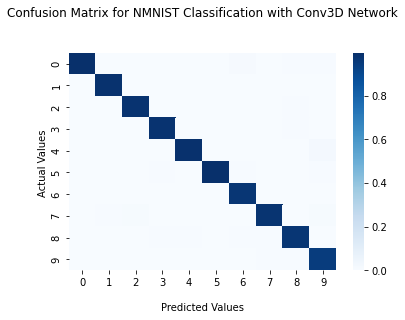
\includegraphics[width=0.4\textwidth]{testingandresults/images/c_matrix_nmnist_conv3d.png}}}%
    \qquad
    \subfloat[\centering]{{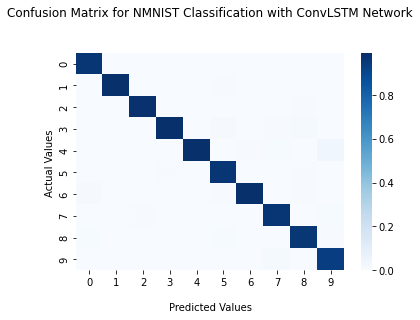
\includegraphics[width=0.4\textwidth]{testingandresults/images/c_matrix_nmnist_convlstm.png}}}%
    \qquad
    \subfloat[\centering]{{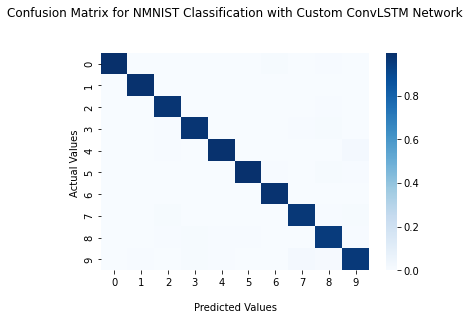
\includegraphics[width=0.4\textwidth]{testingandresults/images/c_matrix_nmnist_custom_convlstm.png}}}%
    \caption{Confusion matrices for the NMNIST classification with various networks; \textbf{(a)} conv3D, \textbf{(b)} convLSTM, \textbf{(c)} custom convLSTM.}%
    \label{fig:nmnist_c_matrices}%
\end{figure}

\color{red} TODO: Make more custom convolution LSTMs \color{black}

\subsubsection{DVS128 Gesture Dataset}

\section{Two-phase Intensity Reconstruction Models}

\subsection{Intensity Reconstruction}

The E2VID reconstruction network (as described in \cref{ssec:video_reconstruction}) was used to recreate intensity videos from events. It was evident that the reconstructions created were robust and relatively to to life. The reconstructions were not effected by adverse lighting effects or fast motions \color{red} TODO: Add image examples \color{black}. This meant that modern computer vision techniques could still be applied to event data, while still preserving the many benefits the event model presents. It was interesting to note the performance of the reconstruction model on inputs with few moving parts. Since events are only triggered when there is an intensity change on any given pixel on the sensor, only regions with motion in them showed up as events, and the nature of all the space with no motion was not easily inferable. This can clearly be seen in \cref{fig:wave_in_lightings_reconstructions}, where only parts of the scene were accurately reconstructed. This did not, however, pose much of a problem for tasks such as gesture recognition, since the motion is exactly what is being classified, however for other tasks such as object recognition it had to be ensured that there was some sort of motion of either the object or the camera for the reconstruction algorithm to be effective.

\color{red} TODO: Include image and explanations of NMNIST reconstructions \color{black}

\Cref{fig:wave_in_lightings_reconstructions} shows that event-cameras do indeed allow for higher fidelity video capture in a wider range of lighting conditions that frame-based cameras (as explained in \cref{ssec:event_camera_benefits}). In all lighting conditions the video reconstruction was largely the same, since the events triggered were very similar in all cases. The logarithmic characteristics of the event-sensor pixels are the reason for this, since the thresholds for the triggering of events is not static. Since the reconstructions are consistent across lighting conditions, this also means that the reconstruction is more reliable, and the classification algorithm works better in adverse conditions in general \color{red} TODO: get figures and images to prove this \color{black}.

\begin{figure}[htb]%
    \centering
    \subfloat[\centering]{{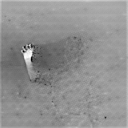
\includegraphics[width=0.18\textwidth]{testingandresults/images/dvs_wave_fluorescent_led.png}}}%
    \qquad
    \subfloat[\centering]{{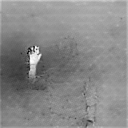
\includegraphics[width=0.18\textwidth]{testingandresults/images/dvs_wave_fluorescent.png}}}%
    \qquad
    \subfloat[\centering]{{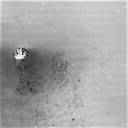
\includegraphics[width=0.18\textwidth]{testingandresults/images/dvs_wave_lab.png}}}%
    \qquad
    \subfloat[\centering]{{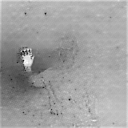
\includegraphics[width=0.18\textwidth]{testingandresults/images/dvs_wave_led.png}}}%
    \qquad
    \subfloat[\centering]{{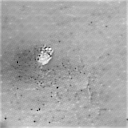
\includegraphics[width=0.18\textwidth]{testingandresults/images/dvs_wave_natural.png}}}%
    \caption{A waving motion being reconstructed from events captures by DVS128 event camera under different lighting conditions.The lighting conditions are as follows; \textbf{(a)} fluorescent led, \textbf{(b)} fluorescent, \textbf{(c)} lab lighting, \textbf{(d)} led lighting and \textbf{(e)} natural lighting.}%
    \label{fig:wave_in_lightings_reconstructions}%
\end{figure}

\subsection{Classification Results}

\subsubsection{NMNIST Dataset}

\subsubsection{DVS128 Gesture Dataset}

\section{Classification Results of All Networks}

\begin{table}[htb]
    \centering
    \begin{tabular}{|| c | c | c ||}
        \hline
        Network     & NMNIST & DVS128 Gesture \\
        \hline \hline
        Conv3D Event Classifier          & 98.22\%   &   52.43\%    \\
        \hline
        Conv2D LTSM Event Classifier         & 97.48\%   &        \\
        \hline
        Custom LTSM Event Classifier         & 97.88\%  &        \\
        \hline
        Conv2D LTSM Reconstruction Classifier           & \color{red} 83.13\% \color{black}    &    \color{red} 19.26\% \color{black}   \\
        \hline
    \end{tabular}
    \caption{A table showing classification accuracies of various models.}
    \label{tab:network_performances}
\end{table}

\begin{table}[htb]
    \centering
    \begin{tabular}{|| c | c | c ||}
        \hline
        Network     & NMNIST & DVS128 Gesture \\
        \hline \hline
        Conv3D Event Classifier          & 1h43m3s   &       \\
        \hline
        Conv2D LTSM Event Classifier         & 1h3m9s   &        \\
        \hline
        Custom LTSM Event Classifier         &    &        \\
        \hline
        Conv2D LTSM Reconstruction Classifier           &     &      \\
        \hline
    \end{tabular}
    \caption{A table showing training times various models.}
    \label{tab:network_training_times}
\end{table}